\hsection{Composite Attributes}%
\hsection{Violation:~{T}he Use of Composite Attributes}%
\FloatBarrier%
%
\begin{figure}%
\centering%
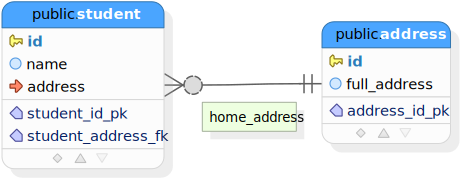
\includegraphics[width=0.85\linewidth]{\currentDir/anomalyComposite}%
\caption{A violation of the \pgls{1NF}:~{T}he \sqlil{full_address} field is semantically a composite attribute, but represented as flat \sqlilIdx{VARCHAR}.}%
\label{fig:anomalyComposite}%
\end{figure}%
%
\gitExecSQLraw{}{}{normalization/1nf/anomaly_composite/generated_sql}{01_anomalies_database_2001.sql}{}{}{}%
%
\gitLoadAndExecSQL{1nf:anomaly_composite:03_public_address_table_5071}{}{normalization/1nf/anomaly_composite/generated_sql}{03_public_address_table_5071.sql}{anomalies}{}{}%
\listingSQL{1nf:anomaly_composite:03_public_address_table_5071}{The generated \sql\ code for creating the \sqlil{address} table that violates the \pgls{1NF} based on \cref{fig:anomalyComposite}.}%
%
\gitLoadAndExecSQL{1nf:anomaly_composite:04_public_student_table_5075}{}{normalization/1nf/anomaly_composite/generated_sql}{04_public_student_table_5075.sql}{anomalies}{}{}%
\listingSQL{1nf:anomaly_composite:04_public_student_table_5075}{The generated \sql\ code for creating the \sqlil{student} table based on \cref{fig:anomalyComposite}.}%
%
\gitExecSQLraw{}{}{normalization/1nf/anomaly_composite/generated_sql}{05_public_student_student_address_fk_constraint_5080.sql}{anomalies}{}{}%
%
\gitLoadAndExecSQL{1nf:anomaly_composite:insert}{}{normalization/1nf/anomaly_composite}{insert.sql}{anomalies}{}{}%
\listingSQL{1nf:anomaly_composite:insert}{
Inserting some data into the tables~\sqlil{student} and~\sqlil{address} in violation of the \pgls{1NF} based on \cref{fig:anomalyComposite}.}%
%
\gitLoadAndExecSQL{1nf:anomaly_composite:select}{}{normalization/1nf/anomaly_composite}{select.sql}{anomalies}{}{}%
\listingSQLandOutput{1nf:anomaly_composite:select}{select.sql}{%
Trying to find all the students with an address in China, which is hard, because table \sqlil{address} violates the \pgls{1NF}.}{}%
%
\gitExecSQLraw{}{}{normalization/1nf/anomaly_composite}{cleanup.sql}{}{}{}%
%
In \cref{fig:anomalyComposite}, we illustrate a part of a logical model that relates student records to address records.
In this relationship, each student has exactly one address.
In \cref{lst:1nf:anomaly_composite:03_public_address_table_5071,lst:1nf:anomaly_composite:04_public_student_table_5075}, we create the two tables, while leaving the \db\ and constraint creation to your imagination.
We then insert some data into them \db\ \cref{lst:1nf:anomaly_composite:insert}.
At first glance, all looks well.

And all could be well, if we would treat the address of a student always as a single text string.
However, this is not necessarily true, especially not true in our teaching management platform example.
In our example, Mr.~Bibbo lives directly in our Hefei University whereas Mr.~Babbo comes from Quanzhou~(泉州市) in the Fujian province~(福建省).
Mr.~Bebbo and Ms.~Bibbi, however, are foreign exchange students~(留学生) from Germany and the USA, respectively.
Assume that this table would be much larger.
What would happen if we wanted to know who of our students have a valid address in China?
How would we do that?%
%
\begin{sloppypar}%
Matter of fact, we encountered this very same situation back in \cref{sec:factory:table:customer:insert}.
Back then, we used the \sqlilIdx{ILIKE} expression and we do so again here:
In \cref{lst:1nf:anomaly_composite:select}, we combine the tables~\sqlil{student} and \sqlil{address} by using an \sqlilIdx{INNER JOIN} statement.
We then only keep the rows \sqlil{WHERE full_address ILIKE '\%china\%'}, in other words, where the word \inQuotes{china} occurs anywhere in the \sqlil{full_address} columns, regardless of its casing.
\inQuotes{China,} \inQuotes{china,} \inQuotes{CHINA,} \inQuotes{cHina} -- all are OK.
Doing this will yield the two students Mr.~Bibbo and Ms.~Bibbi.
Ms.~Bibbi, however, is a foreign exchange student.
She lives in \emph{China}town, New York.
Also, Mr.~Babbo was not listed, as he declared his address to be in the PRC, i.e., the People's Republic of China.%
\end{sloppypar}%
%
We are faced with two problems:
The first one is that we have no method to decide what part of the \sqlil{full_address} is the country and what not.
The second problem is that there are many different ways to declare that the country of an address is China.

The first problem is caused directly by our violation of the \pgls{1NF}.
Here, we did not model the attribute for the address as a composite attribute.
We modelled it as an atomic attribute, which turned out to be wrong, because now we want to access its components.
An atomic attribute does not have components.

Now our \db\ can still \inQuotes{work}.
We can construct the second query in \cref{lst:1nf:anomaly_composite:select}, which deals with both of the special cases mentioned above.
We exclude addresses that have China in their text but also Chinatown.
And we include addresses that mention PRC and, for good measures, also those including P.R.C.
These, however, are only crutches and no solutions.
We can easily imagine addresses that still will be misclassified.
For example, what do we do with the \inQuotes{Embassy of China in Berlin, Germany}?%
\endhsection%
%
\hsection{Repair:~{D}isassembling the Composite Attribute}%
\begin{figure}%
\centering%
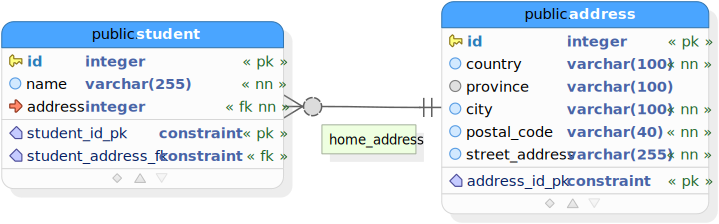
\includegraphics[width=0.85\linewidth]{\currentDir/fixedComposite}%
\caption{A new variant of \cref{fig:anomalyComposite} that does no longer violate the \pgls{1NF}. %
The address data has been disassembled in several columns, allowing us to extract the country of an address with ease.}%
\label{fig:fixedComposite}%
\end{figure}%
%
\gitExecSQLraw{}{}{ normalization/1nf/fixed_composite/generated_sql}{01_fixed_database_2001.sql}{}{}{}%
%
\gitLoadAndExecSQL{1nf:fixed_composite:03_public_address_table_5071}{}{normalization/1nf/fixed_composite/generated_sql}{03_public_address_table_5071.sql}{fixed}{}{}%
\listingSQL{1nf:fixed_composite:03_public_address_table_5071}{%
The generated \sql\ code for creating the \sqlil{address} table based on \cref{fig:fixedComposite}, which no longer violates the \pgls{1NF}.}%
%
\gitExecSQLraw{}{}{normalization/1nf/fixed_composite/generated_sql}{04_public_student_table_5079.sql}{fixed}{}{}%
\gitExecSQLraw{}{}{normalization/1nf/fixed_composite/generated_sql}{05_public_student_student_address_fk_constraint_5084.sql}{fixed}{}{}%%
\gitLoadAndExecSQL{1nf:fixed_composite:insert}{}{normalization/1nf/fixed_composite}{insert.sql}{fixed}{}{}%
\listingSQL{1nf:fixed_composite:insert}{%
Inserting some data into the tables~\sqlil{student} and~\sqlil{address} as designed in \cref{fig:fixedComposite}, which now comply with the \pgls{1NF}.}%
%
\gitLoadAndExecSQL{1nf:fixed_composite:select}{}{normalization/1nf/fixed_composite}{select.sql}{fixed}{}{}%
\listingSQLandOutput{1nf:fixed_composite:select}{select.sql}{%
Trying to find all the students with an address in China becomes easier now, because \sqlil{county} is its own column. %
Also, reassembling the full address using the string concatenation operation~\sqlil{||}\sqlIdx{\textbar\textbar}.}{}%
%
\gitExecSQLraw{}{}{normalization/1nf/fixed_composite}{cleanup.sql}{}{}{}%
%
Let us now fix this problem.
A proper solution can only be to model the address as a composite attribute.
At least the country needs to be split off.
Maybe also the province, because that could come in handy, too.
We probably also want a postal code.
We apply these ideas to create the improved logical model in \cref{fig:fixedComposite}.

The attribute~\sqlil{full_address} now now longer exists when we create the table \sqlil{address} in \cref{lst:1nf:fixed_composite:03_public_address_table_5071}.
Instead, we have the columns~\sqlil{country}, \sqlil{province}, \sqlil{city}, \sqlil{postal_code}, and~\sqlil{street_address}, all of which are of type \sqlilIdx{VARCHAR} of appropriate lengths.
We permit \sqlil{province} to be \sqlilIdx{NULL}, because some countries maybe do not have provinces, whereas all other fields must be~\sqlilIdx{NOT NULL}.
Nothing else changes, the table~\sqlil{student} can stay as it is.

When we insert the data into our \db\ \cref{lst:1nf:fixed_composite:insert}, we of course also need to split the addresses properly over the columns.
This also shows us a slight drawback that is inherent to all normal forms:
They break compound data into independent pieces.
If we later need the complete data again, we need to reassemble the pieces.
Thus, if we need the full address string, we first must reassemble it, probably using the string concatenation operator~\sqlil{||}\sqlIdx{\textbar\textbar}~\cite{PGDG:PD:SFAO}.

As you can see in \cref{exec:1nf:fixed_composite:select}, we now can indeed obtain the list of all students with addresses in China much more easily.
It is a given that we still have to deal with the fact that different people may use different names for the country, but at least we cannot accidentally classify someone from Chinatown in San Francisco as a PRC resident.

While we are here, let's do a small excursion that just fits nicely in this topic but is otherwise unrelated to the \pgls{1NF}.
If you read \cref{lst:1nf:fixed_composite:select}, you notice that reassembling the full address was a bit complicated and went beyond simply using~\sqlil{||}\sqlIdx{\textbar\textbar}.
This is because we allowed the \sqlil{province} column to be \sqlil{NULL}.

We even have such a case in our table:
A new student, Ms.~Bebbe, has joined our university and she is from Beijing~(北京市).
Beijing that does not belong to any province but is a municipality directly under the central government of China.
Therefore, when adding her address record, we left the \sqlil{province} column as~\sqlil{NULL}.

In \postgresql, concatenating a string with \sqlilIdx{NULL} yields \sqlilIdx{NULL}.
If we just combined all the address fields using \sqlil{||}\sqlIdx{\textbar\textbar}, we would yield \sqlilIdx{NULL} for the address of Ms.~Bebbe.
To deal with the potentially \sqlil{NULL} in the \sqlil{province} field, we use the \sqlilIdx{COALESCE} function~\cite{PGDG:PD:CE}.
This function takes arbitrarily many arguments and returns the first argument that is not~\sqlilIdx{NULL}~(or \sqlilIdx{NULL} if all of its arguments are~\sqlilIdx{NULL}).%
%
\begin{sloppypar}%
When reading the query, you will also find one additional change when checking the country:
We could have used the logical \sqlilIdx{OR} to combine the three conditions \sqlil{country ILIKE '\%china\%'}, \sqlil{country ILIKE '\%PRC\%'}, and \sqlil{country ILIKE '\%P.R.C.\%'}\sqlIdx{ILIKE}.
Instead, we wrote \sqlil{country ILIKE ANY(ARRAY['\%china\%', '\%PRC\%', '\%P.R.C.\%'])}\sqlIdx{ANY}\sqlIdx{ARRAY}, which is equivalent to that~\cite{PGDG:PD:RAAC,PGDG:PD:A}:
We can declare an array of the values \sqlil{a}, \sqlil{b}, \sqlil{c}, and~\sqlil{d} as \sqlil{ARRAY[a, b, c, d]}\sqlIdx{ARRAY}.
The expression \sqlil{XXX operator ANY(ARRAY[...])}\sqlIdx{ANY} becomes \sqlil{TRUE} if \sqlil{XXX operator YYY} is \sqlil{TRUE} for any, i.e., at least one, \sqlil{YYY} in the array~\cite{PGDG:PD:RAAC}.
In our case, \sqlil{XXX} is \sqlil{country} and \sqlil{operator} is \sqlilIdx{ILIKE}.
(Similarly, the expression \sqlil{XXX operator ALL(ARRAY[...])}\sqlIdx{ALL} becomes \sqlil{TRUE} if \sqlil{XXX operator YYY} is \sqlil{TRUE} for every single, i.e., all, \sqlil{YYY} in the array~\cite{PGDG:PD:RAAC}.)
Thus, we can use the shorter expression to save a bit space.%
\end{sloppypar}%
%
Anyway, we have seen one anomaly that can occur when designing logical schemas.
If we incorrectly model composite attributes as atomic attributes and later need to pull the components out of them, we can quickly descend into the hell of crutches and special cases.
Properly recognizing the nature of attributes and strictly adhering to the \pgls{1NF} can reduce the potential errors very significantly.
It comes at the cost of slightly more complicated queries when reassembling the compound data.%
%
\FloatBarrier%
\endhsection%
\endhsection%
%
